\section{Introduction}
The goal of this chapter is to review the existing tools for managing
bibliographies and how these tools address the issues covered in
Chapter~\ref{ch:problem-description}.

The chapter is organized as follows: an overview of the pure tools for
{\bibtex} \chapref{sec:bibtex_tools}, some of the attempts to replace
{\bibtex} \chapref{sec:bibtex_alternatives} and bibliography mangers
that strive to redesign how to manage bibliographies
\chapref{sec:bibliography_managers}.


\section{{\bibtex} tools}
\label{sec:bibtex_tools}
There are a few pure {\bibtex} tools for handling reference databases.
Some of these tools target some of the issues described.  The various
tools have either been tested or their functionality verified by code
inspection.

\subsection{Bibcleaner}
Bibcleaner is a tool developed by Joos Buijs for his own use in his
PhD studies and made publicly available in case someone can get a use
for it.  The purpose of the tool is to clean {\bibtex} files by using
online lookups in the DBLP database~\cite{bibcleaner_source,
  bibcleaner_question}.

Bibcleaner is quite simple: it runs through each entry comparing it
with the DBLP database and suggests improvements if it can find the
current key in the database.  The functionality of the tool is
currently limited to computer science, as it only uses DBLP for
lookups~\cite{bibcleaner_source}.

\subsection{BibTooL}
BibTooL is a {\bibtex} that was developed by Charalampos Nikolaou from
University of Athens.  The last version of the tool is from July 2012
and there is no indication of further development being done.  BibTooL
is a set of shell scripts to assist in cleaning, organizing and
ensuring consistency in {\bibtex} files~\cite{bibtool_site}.

The only method for handling of abbreviations in BibTooL is by
DBLP-lookup, like Bibcleaner.  However, unlike Bibcleaner, it also
provides some tools for correcting inconsistencies.  Mostly it is
inconsistencies in the formatting, such as trailing spaces and
capitalization of the entry types (such as @article) together with a
tool for detecting duplicate entries.

\subsection{JabRef}
JabRef is an open source project, currently developed and maintained
by Jörg Lenhard, Matthias Geiger, Oliver Kopp, Simon Harrer and Stefan
Kolb~\cite{jabref_developers}.  It is using the pure {\bibtex} format
and has features for automatic key generation, searching online
databases and a plugin system~\cite{jabref_features}.  There is a
feature for handling Journal Abbreviation using predefined lists of
abbreviations~\cite{jabref_abbreviations}.  Currently, JabRef does not
have any spell checking features, but it is planned for implementation
in the next full release~\cite{jabref_spellchecker}.

The JabRef team is currently working on a tool named CloudRef which
has a focus on a web based interface for collaboration.  Currently,
the project is in the planning phase and suggested features hint that
it might end up correcting some of the issues, as there is some focus
on correctly filled {\bibtex} references and corrections for those.

Looking through the lists of JabRef plugins does not reveal any that
provide solutions to the issues of this dissertation.  There are
plugins for lookups in online databases, which can offer a partial
solution (provided the online information is correct and that it is
there for the reference) for new entries~\cite{jabref_resources}.
Since JabRef uses {\bibtex} for storage, tools for {\bibtex} can be
used too.

When using JabRef, it is very easy to switch between journal
abbreviations and full names, provided that the abbreviation is
already known, with the ability to add custom
abbreviations~\cite{jabref_abbreviations}.  The supposed spell check
was not to be found in the beta release of JabRef.  Doing lookups
online for details can in theory be done during PDF-import using
Mr. DLib, which supposedly should search for entries based on
similarity to \file{PDF}s.  The project seems to be abandoned as the
site has not been updated since
2012~\cite{jabref_mrdlib_notice,jabref_mrdlib}.  It is worth nothing
that JabRef has a system for finding duplicate entries, and does some
validation of {\bibtex} files when opened to ensure valid data.

\subsection{Bibcut}
Bibcut is a tool to arrange and modify {\bibtex} files in ways that
will assist scientists.  It is developed by Dr. Clemens Barth with the
latest release from 2014.  Bibcut can be used to clean author strings
to ensure consistent formatting, compare {\bibtex} files, for instance
to find duplicates and ways of handling journal names and change them
from abbreviations to full names or vice versa~\cite{bibcut_site}.

\subsection{{\bibtex} Check}
{\bibtex} Check was developed by Fabian Beck to validate if required
fields are present, to do consistency checks on conference proceedings
and to provide an easy overview in html with links to relevant sources
such as Google Scholar and DBLP.

The way {\bibtex} Check works is by running some very simple checks to
find flaws in bibliographies.  The checks are things like: check if
the value for $author$ contains a period(.), to find initials, check
that the mandatory fields are present, and check if an entry contains
fields from another entry type.  For instance, if a $@PROCEEDINGS$
contains the $pages$ tag, to suggest that the user might have meant
$@INPROCEEDINS$ instead.


\section{{\bibtex} alternatives}
\label{sec:bibtex_alternatives}
There are both variants of and alternatives to {\bibtex}.  A quick
overview of a few of the options is provided.  Mostly they do not
provide many new options.

\subsection{{\bibtex}ml} {\bibtex}ML is a version of {\bibtex} where
the entries are formatted with XML.  It is by design made with strict
schemas and conversion tools to convert from {\bibtex}.  Having a
system using strict schemas enables enforcing correct entries that
conform to the specification.  The strict approach will prevent usage
of non-conforming tags.  On the down side, this approach also makes it
hard to introduce new de facto standards when they are
needed~\cite{gunhen2007_bibtexml}.

\subsection{MLBIBTEX}
MLBIBTEX is an variant of {\bibtex} from Jean-Michael Hufflen to
create support for multiple languages.  The focus of MLBIBTEX is to
add support for entries in different languages, accounting for
appropriate naming of language specific content (such as months).
This variant has been made to account for authors writing in different
languages, such as a lecturer writing course material for students in
their native language.  It does not seem that MLBIBTEX takes care of
the issues that arise from the lack of encoding support in
{\bibtex}~\cite{hufflen2001_mlbibtex}.


\subsection{Bib{\LaTeX} and biber}
\label{sec:related_biblatex}

Bib{\LaTeX} is a {\LaTeX} package intended to replace {\bibtex}, but
with backward compatibility with {\bibtex}.  It is designed to be able
to run with the {\bibtex} backend, but defaults to use biber instead.
The idea behind Bib{\LaTeX} and biber is to overcome some of the
limitations of {\bibtex}, such as the limited character support,
limited options for sorting and the need for new entry types (for
instance, {\bibtex} does not have an entry for online resources).
Most notably, the Bib{\LaTeX} and biber combination adds the support
for mappings of the entry content, for instance, to ensure that journal
names get abbreviated when printing the bibliography.


\section{Bibliography managers}
\label{sec:bibliography_managers}

Bibliography managers, sometimes also called reference managers, are
software tools for bibliography management that are not directly
targeted at {\bibtex}.  Some of these provide partial solutions for
the lexical and consistency concerns.  All of the tools have been
tested for relevant features that are not described on their
respective feature overviews.

\subsection{Mendeley}
\label{sec:related_mendeley}

Mendeley is a bibliography management tool developed by Mendeley Ltd.
The focus of the tool is to make it easy to manage and share
references.  Mendeley provides features such as importing \file{PDF}s
and detecting relevant details such as the author, title and DOIs, and
updating entries from online databases using, for instance, the DOI.
The target group for Mendeley is students and
researchers~\cite{mendeley_features}.

Like {\bibtex}, Mendeley does not facilitate any systems for detecting
inconsistencies such as spelling errors, revision numbers or initials.
Mendeley can download meta-information based on a DOI which in part
remedies the lack of these tools.  Mendeley does not have any
plugin/add on system, so it's unlikely that there are any third party
tools to further handle the {\bibtex} issues. A search through
Mendeley's request database reveals the same as the testing and
features page.  On Mendeleys online request system, there are requests
for features such as: spell checking, fixing capitalization
inconsistencies and bulk DOI lookups~\cite{mendeley_request_bulk_doi,
  mendeley_request_capitalization, mendeley_request_spellcheck,
  mendeley_request_lowercase}.

\subsection{EndNote and RefMan}
EndNote and RefMan are also tools for reference mangement, made by
Thompson Reuters.  RefMan is an older product and Thompson Reuters
recommends using EndNote instead~\cite{refman_switch,
  refman_features}.  The focus is on: the sharing capabilities, tools
for PDF import and management, online lookup of references and
detection of journal abbreviations~\cite{endnote_basic_features,
  endnote_x7_features}.  Their target group is students and university
related groups.  EndNote also provides a spell check feature that is
not mentioned in the feature sets~\cite{endnote_spellcheck}.

The tool for handling abbreviations in EndNote is only used to format
the names when exported or used as references.  This is done using a
mapping from a predefined set of known abbreviations, not fixing the
naming issues internally in the files~\cite{endnote_terms_journals}.

When trying to remedy the spelling and consistency errors by using DOI
lookups, it seems that the only way of doing that will create
duplicate entries rather than updating the current one. This is just
making the issues even worse, as the references then end up with
duplications too.  The spell checker works on a per entry basis and
there is no apparent way to spell check an entire bibliography.
EndNote provides of extra downloads to provide features such as
{\bibtex} support.  However no downloads were found to remedy neither
the lexical nor the consistency concerns
further~\cite{endnote_downloads}.


\subsection{Zotero}

Zotero is a bibliography manager developed by Roy Rosenzweig Center
for History and New Media.  It is targeted at people doing research.
The organization and collaboration aspects are in focus for
Zotero~\cite{zotero_features}.

There is a built in spell checker for notes written in Zotero.
However the spell checker is not applied for things like titles, which
prevents it from detecting those errors.  Like JabRef, Zotero has a
plugin system.  Plugins to remedy the {\bibtex} issues is neither
found using the official list of plugins~\cite{zotero_plugins} nor by
a normal search engine. There is a limited mechanism for detecting
abbreviations in Zotero, in its \file{jar} there is a list of known
abbreviations which it can use to choose the correct abbreviation when
exporting.  Entering an abbreviation does not seem to correct it to
the non-abbreviated version.  This list can be manually edited, and
overruled~\cite{zotero_abbreviations}.

It is possible (but not tested) that Zotero can be used to import a
{\bibtex} file, then export it using the lists of known abbreviations
and correct the abbreviations already known.  As other tools, such as
JabRef and Mendeley, already allow this procedure, we did not test for
this feature.


\subsection{RefWorks}
RefWorks is a web based bibliography manager developed by ProQuest,
meant for students, researchers and librarians.  The focus of the tool
is to have the simplicity of a web based solution, which makes the
resources easy to share and available everywhere.  The features
include online lookups, statistics systems and collaboration
features~\cite{refworks_features}.

As with the other tools, testing shows that the error detection
features are limited.  In RefWorks, the work flow for adding
references is to either enter them manually or to use a browser link
called ``RefGrab-It'' to import from homepages.  RefGrab-It can be
used for DOI lookups, which enables the same advantages as Mendeey and
EndNote.  Contrary to the other tools, RefWorks tries to detect if the
author name is malformed, although it only seems to detect if one
types ``John Doe'' rather than ``Doe, John'' as it expects, as can be
seen at Figure~\ref{fig:refworks-detect-formatting}.

\begin{figure}
    \centering
    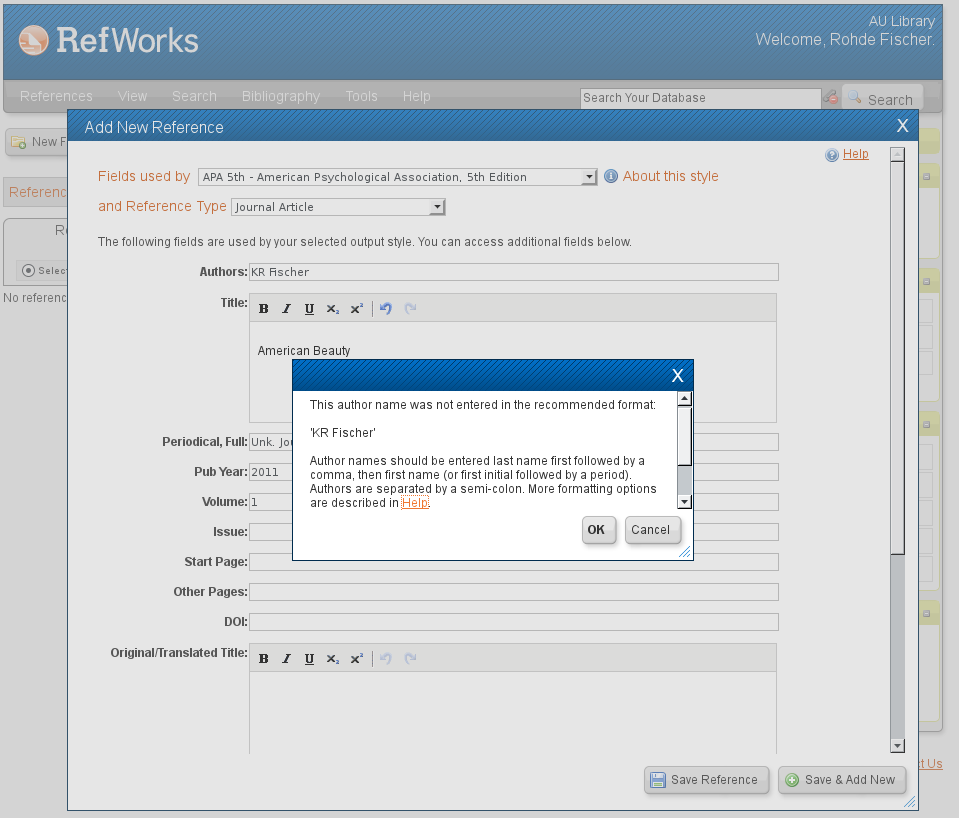
\includegraphics[width=0.85\textwidth]{refworks-detect-formatting}
    \caption{RefWorks detects some formatting on the name field}
    \label{fig:refworks-detect-formatting}
\end{figure}

In RefWorks itself there seems to be no spell checker, but the
spelling errors are in part solved by most modern browsers, because
they often include a spell checker for input fields.

\subsection{Papers}
Papers is a bibliography manager developed by Mekentosj B.V., targeted
for science and research.  It provides a tool set for searching online
libraries for references, collaboration and various ways of
organizing~\cite{papers_features}.

It does not highlight any features of relevance~\cite{papers_features}
and as it is developed for Mac OS, it has not been possible to test if
there is relevant features apart from what they mention on their page.

%\subsection{ALICE}
%ALICE is an abbreviation detection system for bio articles. It uses a
%lot of rules to detect abbreviation styles.

%Perhaps some of those rules can be reused in my project?


\section{Summary and conclusions}
There are various ways to handle bibliographic references.  Right from
a multitude of tools that strive to assist with maintenance of one's
{\bibtex} library, alternatives to {\bibtex} and bibliography managers
that strive to replace the entire management process.  Some of these
help by doing online lookups to double check entries, finding
duplicates, assisting in transforming to and from abbreviated forms,
enforcing strict rules and spell checking.

Some of these tools do provide partial solutions to the issues with
{\bibtex}, but none of them provide complete solutions and none of
them combines the solutions into a more general solution.  The pure
{\bibtex} tools can of course be combined.  Since Bib{\LaTeX} is
designed to be close to {\bibtex}, there is a chance that some of the
{\bibtex} tools work on Bib{\LaTeX} too (which has not been tested).
The alternative formats provide some ways to gain strict conformity
and to manage abbreviations, but apart from that, not much
consolidation on the issues.  The reference managers in general focus
on the collaboration between authors.  Only a few of the tools provide
assistance with the issues, such as spell checking and abbreviation
handling.

Having seen approaches to the {\bibtex} issues and having reviewed how
others approach them.  How can one analyze {\bibtex} files, to detect
these issues?  In the next chapter our suggestion for analyzing is
covered.


%%% Local Variables:
%%% mode: latex
%%% TeX-master: "thesis"
%%% End: